\chapter{声音如何传播}\label{ch:g4:how-sound-travels}

闪电的一闪 --- 随后是一、二、三秒的寂静
--- 这时才传来雷的隆隆声。可是闪电和雷声
其实诞生于同一片云中！我们已经知道，声音是一种颤动，
它会传播。本章将沿着它的路径，探讨它传播经过什么、
传播得多快，以及遇到墙壁时会发生什么。

\section{声音需要介质}

\begin{proposition}[没有介质，就没有声音]\label{prop:g4:how-sound-travels:carrier}
声音只能\emph{通过}某些物体传播：通过空气、通过
水、木头、砖和钢铁。若什么都没有，
——没有空气，也没有任何物质——声音便无法传播：
颤动便无物可以颤动。
\end{proposition}

\begin{example}[玻璃罩中的电铃]\label{ex:g4:how-sound-travels:jar}
一个著名的实验，已有三百年历史：电铃在玻璃罩内响着，
声音清晰可闻。随后，抽气泵把密封罩内的空气抽出，
同时可见电铃的锤子仍在不停地敲击。
铃声渐弱……直至消失。放入空气，
铃声便又回来。电铃其实从未停止，它的\emph{介质}
被抽走又放回。现在，可以解答一个古老的疑问：
月球上没有声音，那里即使大喊也无人听见，之所以寂静无声，是因为它
根本没有空气。
\end{example}

\begin{omfigure}
\begin{tikzpicture}[scale=0.85]
  \draw[thick] (0.7,0) -- (0.7,3.0) .. controls (0.7,3.5) and
    (3.3,3.5) .. (3.3,3.0) -- (3.3,0);
  \draw[thick] (0.2,0) -- (3.8,0);
  % the bell: hanger, dome with a flared skirt, mouth, clapper
  \draw[thick] (2.0,2.9) -- (2.0,2.45);
  \draw[thick, fill=yellow!65!orange]
    (1.42,1.52)
    .. controls (1.5,1.6) and (1.58,1.7) .. (1.6,1.85)
    .. controls (1.62,2.1) and (1.65,2.45) .. (2.0,2.45)
    .. controls (2.35,2.45) and (2.38,2.1) .. (2.4,1.85)
    .. controls (2.42,1.7) and (2.5,1.6) .. (2.58,1.52)
    -- cycle;
  \draw[thick] (1.42,1.52) .. controls (2.0,1.43) .. (2.58,1.52);
  \fill (2.0,1.38) circle (0.07);
  \draw[omDef, dotted, thick] (1.15,1.9) arc (150:210:0.5);
  \draw[omDef, dotted, thick] (2.85,2.15) arc (30:-30:0.5);
  \node[right, font=\small] at (4.3,2.6) {密封玻璃罩};
  \node[right, font=\small] at (4.3,1.8) {电铃仍在敲击};
  \node[right, font=\small] at (4.3,1.0)
    {抽去空气：铃声消失};
  \draw[-Stealth, thick, omExo] (3.0,0.35) -- (4.1,0.35);
  \node[right, font=\small, omExo] at (4.15,0.35) {通往抽气泵};
\end{tikzpicture}

{\small 罩中的电铃：抽走空气，停止的是声音
——而不是电铃。}
\end{omfigure}

\begin{example}[比空气更好的介质]\label{ex:g4:how-sound-travels:solids}
固体和水传播声音的能力出色——往往比空气还好。
把耳朵紧贴在桌面上，请朋友轻轻刮擦远端，
通过空气你什么也听不到；\emph{很}轻地刮擦，通过
木头，刮擦声清晰响亮。游泳者能听见泳池水下
从一端到另一端的敲击声；鲸鱼能隔着
整片海洋彼此呼应。厚厚的墙壁会把邻居的钻孔声传入
每个房间——固体在这方面几乎好得过了头。
\end{example}

\begin{method}[线电话]\label{met:g4:how-sound-travels:telephone}
\begin{enumerate}
  \item 在两只纸杯的杯底各戳一个小孔；
  \item 将长线的两端穿入小孔，并在每端打结，
        使其不会滑出；
  \item 两人走开，直到线被拉得\emph{很紧}，并且
        途中不碰到任何东西；
  \item 一人轻声对着纸杯说话，另一人把纸杯
        贴在耳边。
\end{enumerate}
低语声清晰地传过操场：你的声音使纸杯
颤动，颤动沿着绷紧的线传播，于是
远处的纸杯把它重现出来。若线松弛下垂，或用两根手指捏住它，
电话便失效了——传播的路径被切断。
\end{method}

\begin{omfigure}
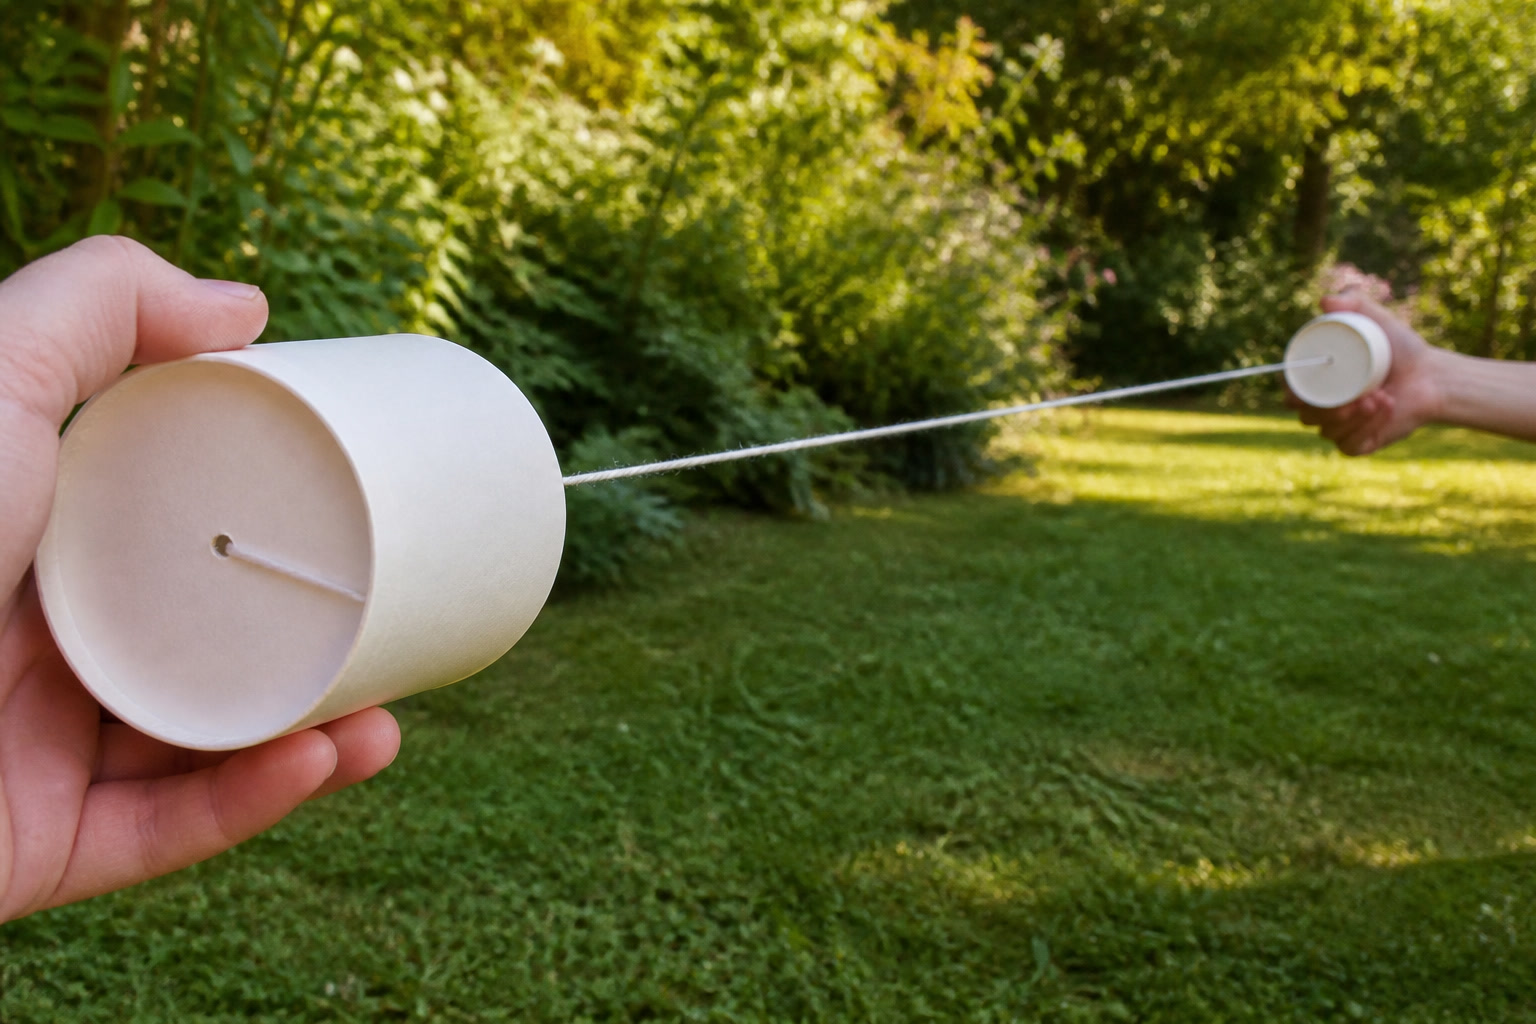
\includegraphics[width=0.58\linewidth]{images/book1/ai/g4-sound-string-telephone.jpg}

{\small 拉紧的线电话：绷紧的线传递颤动，远比两人之间的空气效果好得多。}
\end{omfigure}

\section{声音需要时间}

\begin{proposition}[很快，但并非瞬间]\label{prop:g4:how-sound-travels:speed}
声音是个奔跑者，而不是魔术师：在空气中，它每秒约传播
\qty{340}{m}——大约一千米需要三秒。
相比之下，光到达得极快，在任何可观察的场景中，
它的传播都可视为瞬间完成。这一差异
正是雷暴现象的全部缘由。
\end{proposition}

\begin{method}[雷暴有多远？]\label{met:g4:how-sound-travels:storm}
\begin{enumerate}
  \item 看到闪光——开始匀速数秒：一
        只小鳄鱼，两只小鳄鱼，\dots；
  \item 听到第一声雷的隆隆声时停止；
  \item 用计数除以 $3$：所得大约是雷暴的
        距离，单位为千米。
\end{enumerate}
六秒：约 \qty{2}{km}。相邻两次闪击之间
计数越来越短，说明雷暴正在靠近——该回室内了。
\end{method}

\begin{omfigure}
\begin{tikzpicture}[scale=0.85]
  \draw[thick] (0,0) -- (11,0);
  \draw[very thick, omThm] (1.3,3.4) -- (0.9,2.5) -- (1.25,2.5)
    -- (0.8,1.5) -- (1.15,1.5) -- (0.7,0.4);
  \fill[omExo, opacity=0.3] (0.3,3.4) ellipse (1.5 and 0.45);
  % the listener, counting the silent seconds
  \fill (9.6,1.32) circle (0.18);
  \draw[thick] (9.6,1.14) -- (9.6,0.55);
  \draw[thick] (9.6,1.02) -- (9.33,0.75);
  \draw[thick] (9.6,1.02) -- (9.87,0.75);
  \draw[thick] (9.6,0.55) -- (9.4,0);
  \draw[thick] (9.6,0.55) -- (9.8,0);
  \foreach \r in {0.7, 1.4, 2.1} {
    \draw[omDef, thick] (1.0,0.4) ++(\r,0) arc (0:40:\r);
    \draw[omDef, thick] (1.0,0.4) ++(\r,0) arc (0:-12:\r);
  }
  \node[font=\small, align=center] at (9.15,2.35)
    {“\dots{}五、六”\\--- 约 \qty{2}{km}};
  \node[right, font=\small, omDef] at (3.6,0.75)
    {隆隆声以每秒 \qty{340}{m} 的速度传播};
\end{tikzpicture}

{\small 先见闪光，后闻雷声：光几乎瞬时到达，声音
以每秒 \qty{340}{m} 的速度传播。无声的秒数
可用来测量距离。}
\end{omfigure}

\begin{example}[回声]\label{ex:g4:how-sound-travels:echo}
对着田野另一边的大山崖或孤零零的房子大喊：
“喂！”——片刻寂静——“喂！”回应着你自己的
声音。声音碰到大而硬的墙壁会被反弹；反弹后
晚到得足以与原声分开听清的声音，叫做
\emph{回声}\index{回声}。墙壁越远，你的声音往返所用的时间越长，回声便越晚。
在小房间里，反弹声
回来得太快，无法单独听出——它只会让你的声音
听起来更饱满。
\end{example}

\begin{remark}[声呐：被利用起来的回声]\label{rem:g4:how-sound-travels:sonar}
船只测量海水深度时，向下发出一声咔嗒声，
并计算海底回声返回的时间。深水处回声晚，浅水处回声早。
海豚和蝙蝠天生就懂得这一招：它们发出咔嗒声并倾听，
通过读取回声，在昏暗的水中和漆黑的洞穴里搜寻食物。
数雷声的秒数时，
你其实已经用过它们的方法：测出声音的时间，就能知道
距离。
\end{remark}

\section{练习}

\begin{exercise}[$\star$]\label{exo:g4:how-sound-travels:1}
说出本章提到的三种声音的传播介质，
以及一个声音完全无法传播的地方。
\end{exercise}

\begin{exercise}[$\star$]\label{exo:g4:how-sound-travels:2}
在罐子实验中，铃锤仍在不断敲击，而铃声
逐渐消失。究竟被拿走了什么，
这能证明什么？
\end{exercise}

\begin{exercise}[$\star$]\label{exo:g4:how-sound-travels:3}
为什么月球是一个无声的世界？
请用本章的命题作答。
\end{exercise}

\begin{exercise}[$\star$]\label{exo:g4:how-sound-travels:4}
在线电话中，什么传递了低语声？请给出
保持电话正常工作的两条规则。
\end{exercise}

\begin{exercise}[$\star$]\label{exo:g4:how-sound-travels:5}
声音在空气中一秒钟大约能传播多远？
三秒钟呢？
\end{exercise}

\begin{exercise}[$\star$]\label{exo:g4:how-sound-travels:6}
你数出闪光与雷声之间相隔 9 秒，雷暴
离你有多远？你的朋友在下一次闪击时只数了 3 秒——
发生了什么变化？你们俩该怎么办？
\end{exercise}

\begin{exercise}[$\star$]\label{exo:g4:how-sound-travels:7}
为什么把耳朵贴在桌子上，就能听到一声
刮擦声，而它并不是通过空气传来的？
\end{exercise}

\begin{exercise}[$\star$]\label{exo:g4:how-sound-travels:8}
什么是回声？为什么更大、更远的山崖
比近处的山崖回应得晚？
\end{exercise}

\begin{exercise}[$\star$]\label{exo:g4:how-sound-travels:9}
船只的声呐如何区分深水与浅水？哪两种
动物玩着同样的游戏，它们在哪里？
\end{exercise}

\begin{exercise}[$\star\star$]\label{exo:g4:how-sound-travels:10}
老式西部片里常见侦察兵把耳朵贴在钢轨上，
以听取仍然遥远的火车声。为什么钢轨比空气更早
暴露火车的到来？请给出钢轨在传声方面的两个优势。
（其一与传导得好有关；至于另一个，请记住钢轨
是笔直地通向火车，而空气中的声音像池塘里的
水波一样向四面八方扩散，并越传越弱。）
\end{exercise}

\begin{exercise}[$\star\star$]\label{exo:g4:how-sound-travels:11}
站在一个空旷的大院子里，你拍了一次手，
听到拍手声从远处墙壁返回，恰好过了整整一秒。
声音在这一秒内跑到墙壁又回来。墙壁离你
有多远？——注意，要考虑往返路程！
\end{exercise}
